%#################################################################################
	%beginning
	\documentclass[12pt, a4paper]{scrreprt}
	
	%Worttrennung Deutsch
	\usepackage[ngerman]{babel}
	
	%Trennung von Umlauten
	\usepackage{fontspec}
	
	%Zeilenabstand
	\usepackage{setspace}
	
	%Moderne Schrift
	\usepackage{lmodern}
	\setmainfont[Ligatures=TeX]{Arial}
	\renewcommand*\familydefault{\sfdefault}
	
	%Bilder
	\usepackage{graphicx}
	\usepackage{float}
	
	%Quellen
	\usepackage[backend=bibtex,backref=true,sorting=ynt,useauthor=true,]{biblatex}
		
	%Formeln
	\usepackage{amsmath}
		
	%Clever Reference
	\usepackage{hyperref}
	\usepackage[capitalise]{cleveref}
	
	%Quellcode
	\usepackage{listings}
	\usepackage{xcolor}
	\lstset{language=python,
		basicstyle=\footnotesize\ttfamily,
		keywordstyle=\color{blue},
		stringstyle=\color{green},
		commentstyle=\color{red}
		}
	
	%Einrückungen
	\usepackage{parskip}
	
	%Variablen
	\newcommand{\Titel}{Information Retrieval}
	\newcommand{\Autor}{Jesse-Jermaine Richter, Jonas Seng}
	
	%Literaturverzeichnis
	\bibliography{lit.bib}
	
	%Multiline Kommentare
	\usepackage{verbatim}
	
	%Header/Footer
	\usepackage{totpages}
	\usepackage[includeheadfoot, left=2.5cm, top=1.5cm, bottom=1cm]{geometry}
	
	\usepackage{fancyhdr}
	
	\lhead{\nouppercase{\leftmark}}
	\chead{}
	\rhead{\nouppercase{\rightmark}}
	\lfoot{\Titel}
	\cfoot{}
	\rfoot{Seite \thepage\ von 48}
	\renewcommand{\headrulewidth}{0.2pt}
	
	\fancypagestyle{plain}{
		\fancyhf{}
		\renewcommand{\headrulewidth}{0pt}
		\lfoot{\Titel}
		\rfoot{Seite \thepage\ von 40}
	}

	\usepackage{afterpage}
	
	\newcommand\blankpage{%
		\null
		\thispagestyle{empty}%
		\addtocounter{page}{-1}%
		\newpage}
	
	\newtheorem{defi}{Definition}[chapter]
	
%#################################################################################
%#################################################################################

%DOCUMENT BEGIN
\begin{document}	
%---------------------------------------------------------------------------------
		\begin{titlepage}
		
		\centering
		{\Large\bfseries \Titel \par}
		\vspace{2cm}
		Seminararbeit \par
		\vspace{3cm}
		
		des Studienganges Angewandte Informatik \par
		an der Dualen Hochschule Baden-Württemberg Mannheim \par
		\vspace{3cm}
		
		von \par
		\vspace{0.5cm}
		{\itshape \Autor \par}
		\vspace{2cm}
		27.08.2018 \par
		
		\vspace{6.5cm}
		\begin{tabular}{llll}
			Matrikelnummer, Kurs: & & & 8787549/1980179, TINF16AIBI\\
			Ausbildungsfirma: & & & DZ BANK AG, Frankfurt\\
			Betreuer der Ausarbeitung: & & & Herr Prof. Dr. Karl Stroetmann
		\end{tabular}
	\end{titlepage}
	\thispagestyle{empty}
%---------------------------------------------------------------------------------			
	\section*{Erklärung}
	Ich versichere hiermit, dass ich meine Projektarbeit mit dem Thema: \glqq\Titel\grqq{ }selbstständig verfasst und keine anderen als die angegebenen Quellen und Hilfsmittel benutzt habe.

Ich versichere zudem, dass die eingereichte elektronische Fassung mit der gedruckten Fassung übereinstimmt.\\\\\\\\\\\\
\renewcommand{\arraystretch}{0.5}
\begin{tabular}{l@{\hspace{4cm}}l@{\hspace{4cm}}l@{\hspace{4cm}}l}
	\cline{1-1} \cline{3-3} \\
	Ort, Datum && Unterschrift & \\
\end{tabular}
	\thispagestyle{empty}
	\newpage
%---------------------------------------------------------------------------------
	\begin{abstract}
		\begin{spacing}{1,6}
	In diesem Praxisbericht wird das Thema \glqq\Titel\grqq\ behandelt. Hierbei soll der Leser ein Überblick bekommen, was Monitoring ist, welche Vorteile es birgt, ob es sich um ein notwendiges Werkzeug zur verlässlichen Bereitstellung von IT-Sevices handelt und ob es Alternativen gibt. Außerdem wird ein praktischer Teil präsentiert, in welchem ein Quellcode gezeigt wird, der die Teilimplementierung eines Monitoring-Systems widerspiegelt. Hier werden Daten für eine Statusmail verarbeitet und visualisiert.
	
	This practical report deals with the topic \glqq\Titel\grqq . The reader should get an overview of what monitoring is, what advantages it offers, whether it is a necessary tool for reliable provision of IT services and whether there are alternatives. In addition, a practical part is presented in which a source code is shown that reflects the partial implementation of a monitoring system. Data for a status mail is processed and visualized here.
\end{spacing}

	\end{abstract}
	\afterpage{\blankpage}
%---------------------------------------------------------------------------------			
	\tableofcontents
	\thispagestyle{empty}
%---------------------------------------------------------------------------------			
	%Abbildungsverzeichnis
	\listoffigures
	\thispagestyle{empty}
%---------------------------------------------------------------------------------			
	\chapter*{Abkürzungstabelle}
	\label{abkürzung}
	\renewcommand{\arraystretch}{1.5}
\begin{center}
	\begin{tabular}{|l|l|}\hline
		\multicolumn{1}{|c|}{\textbf{Abkürzung:}} & \multicolumn{1}{c|}{\textbf{Bedeutung:}} \\ \hline
		ASCII & American Standard Code for Information Interchange \\ \hline
		DF & Document Frequency \\ \hline
		IDF & Inverse Document Frequency \\ \hline
		IR & Information Retrieval \\ \hline
		PDF & Portable Document Format \\ \hline
		TF & Term Frequency \\ \hline
		TF-IDF & TF-IDF-Maß \\ \hline
	\end{tabular}
\end{center}

	\thispagestyle{empty}
%---------------------------------------------------------------------------------
	\chapter{Einleitung}
	\label{einleitung}
	\section{Was ist Information-Retrieval?}
Information-Retrieval (IR) beschreibt das Bereitstellen spezieller Informationen aus einer großen und unsortierten Datenmengen. Dieses Themengebiet fällt unter Informatik, Informationswissenschaften sowie Computerlinguistik und ist ein wesentlicher Bestandteil von Suchmaschinen wie zum Beispiel Google.
\\
Das Thema besitzt bereits seit einigen Jahren eine hohe, aber dennoch steigende Relevanz. Die Gründe der hohen Relevanz von IR liegen vor allem beim Einsatz von Suchmaschinen. Diese sind in Zeiten des Internets die wohl wichtigste Form der Informationsbeschaffung. Aufgrund der immer schneller steigenden Informationsmengen wird das Thema künftig weiter an Relevanz gewinnen. Unternehmen und Privatanwender wird eine immer wachsende Menge von Informationen zugänglich, die organisiert werden muss, damit relevante bzw. spezifisch gesuchte Informationen jederzeit und ohne Verzögerung gefunden werden.
\\
Um das Ziel der Bereitstellung von Informationen gewährleisten zu können, wird erst eine Durchsuchung und Gewichtung sämtlicher Informationen bzw. Dokumente, die später gefunden werden sollen, durchgeführt. Das zentrale Objekt der Informationsrückgewinnung stellt der invertierte Index dar, dessen Aufbau und Funktionsweise in den nächsten Kapiteln ausführlich erläutert wird. Im Verlauf dieser Arbeit wird die Komprimierung des Indexes sowie das TF-IDF-Maß, welches zur Beurteilung der Relevanz eines Dokumentes genutzt wird, im Fokus stehen.
\\
Die theoretischen Hintergründe des invertierten Index, der Komprimierung und des TF-IDF-Maß werden durch eine Beispiel-Implementierung einer lokalen Suchmaschine in Programmiersprache Python veranschaulicht.

\section{Ziel der Arbeit}
Ziel der Arbeit ist es, ein grundlegendes Verständnis des Themenkomplexes Information-Retrieval zu vermitteln. Das umfasst auch die theoretischen Hintergründe, die für die später vorgestellten Beispielimplementierungen notwendig sind.
\\
Die Beispielimplementierung soll hauptsächlich die folgenden Themengebiete umfassen:\\
\begin{itemize}
	\item Aufbau eines invertierten Indexes
	\item Approximierende Beurteilung der Relevanz eines gefundenen Dokuments mittels tf-idf
	\item Komprimierung des invertierten Indexes
\end{itemize}
Die in dieser Arbeit vorgestellte Implementierung hat nicht den Anspruch auf eine hohe Performance, vielmehr dient diese dem Zwecke der praxisnahen Veranschaulichung der Funktionsweise von IR-Systemen.

\section{Stand der Forschung}
Dieser Abschnitt umreißt kurz den aktuellen Stand der Forschung. Dazu werden zwei Modelle von Information Retrieval knapp beschrieben, die für die Entwicklung einer lokalen Suchmaschine, von Bedeutung sind. Es wird jedoch nur auf ein Modell im Verlauf dieser Arbeit eingegangen.
\\

\subsection{Vector Space Model}
Das Vector Space Model, zu deutsch Vektorraummodell, repräsentiert Dokumente und Anfragen als hochdimensionale, metrische Vektoren \cite{VR_Retrieval}.
Der Anfrage-Vektor wird beim Retrieval-Prozess mit den Dokumenten-Vektoren verglichen. Dabei werden jedoch nur Dokumente betrachtet, welche mit der Anfrage in Verbindung stehen \cite{klass_IR}. Welche Dokumente betrachtet werden, wird mithilfe des invertierten Index ermittelt.
\\
Es gibt verschiedene Maße, mit denen die Vektoren miteinander verglichen werden. Der einfachste Ansatz besteht darin, den Abstand zu berechnen, jedoch ist dies kein sehr gutes Maß. Besser und weit verbreitet ist deshalb das Cosinus-Maß (oder Kosinus-Ähnlichkeit), welches den Winkel zwischen Anfrage-Vektor und Dokumenten-Vektor angibt. Je kleiner der Winkel zwischen den Vektoren, desto höher ist die Relevanz des Dokuments \cite{IR_Uni_Duisburg}.
\\
Dieses Modell wir im Rahmen dieser Arbeit genauer beleuchtet und als Grundlage für die Beispielimplementierung genutzt.

\subsection{Probabilistische Ansätze}
Probabilistische Ansätze basieren auf Wahrscheinlichkeiten. Hierbei wird eine Abschätzung der Wahrscheinlichkeit berechnet, mit der ein Dokument $d$ bezüglich einer Anfrage $q$ relevant ist \cite{IR_Uni_Duisburg}. Zur Abschätzung der Wahrscheinlichkeit gibt es verschiedene Ansätze, die hier jedoch nicht weiter thematisiert werden. Bei allen praktisch nutzbaren Ansätzen sind jedoch eine - je nach Ansatz - große oder kleine Menge von Zusatzinformationen über die Dokumentenkollektion nötig \cite{IR_Uni_Duisburg}.
%---------------------------------------------------------------------------------
	\chapter{Information Retrieval - Theoretische Grundlagen}
	\label{grundlagen}
	\section{Problemstellung}
Wie in der Einleitung bereits angemerkt, beschreibt \glqq Information Retrieval\grqq das Bereitstellen spezieller Informationen aus einer meist großen, unsortierten Datenmenge. Dabei bekommt das System eine vom Nutzer gestellte Abfrage, auch Query genannt, und versucht auf dessen Basis, Daten, die meist als Dokumente vorliegen, zurückzuliefern. Im Gegensatz zu Abfragen im Datenbankumfeld beinhaltet die Query jedoch keinerlei Informationen, um ein spezielles Element eindeutig identifizieren zu können. Dies soll ein IR-System auch nicht leisten. Vielmehr sollen Ergebnisse zurückgeliefert werden, die mit hoher Wahrscheinlichkeit Relevanz bzgl. der gestellten Query besitzen. Der Nutzer selektiert dann die für diesen nötigen Dokumente.
\\
Mathematisch lässt sich dies folgendermaßen formulieren: Aus einer Dokumentenmenge $D$ soll mithilfe einer Funktion eine Teilmenge $D_1$ von $D$ ermittelt werden, die relevant für eine Abfrage $q$ ist.
\\
Um diese Funktion sinnvoll definieren zu können, muss jedoch zuvor die Menge aller Queries, sowie die Menge aller Tokens definiert werden:
\begin{defi}[Menge aller Terme]\label{def:MaT}
	Sei $d \in D$ ein Dokument. Die Menge $T_d$ ist nun die Menge aller Wörter, die in dem Dokument $d$ enthalten sind: $T_d$ = $\{$$t_1$, .., $t_n$$\}$.
	\\
	Die Menge $T$ ist die Menge aller Terme, die in den Dokumenten aus $D$ vorkommen, also:
	$T$ = $T_{d1} \cup .. \cup T_{d_i}$ mit $i \in N$ und $d_i \in D$.
\end{defi}
Mithilfe der Definition \ref{def:MaT} kann nun die Menge aller möglichen Queries definiert werden:
\begin{defi}[Menge aller möglichen Queries]\label{def:MamQ}
	$Q \subseteq 2^T$
\end{defi}
\begin{defi}[Retrievalfunktion]\label{def:RFunktion}
	Eine Funktion $f$: $Q \rightarrow D_1$ heißt Retrievalfunktion, wobei $D_1 \subseteq D$ gilt und $Q$ die Menge aller Queries ist.
\end{defi}
Nachdem die Problemstellung formuliert ist, muss eine Strategie entwickelt werden, wie die Retrievalfunktion nach \cref{def:RFunktion} dargestellt bzw. umgesetzt wird.
\\
\section{Strategiefindung}
Dieser Abschnitt bietet eine Übersicht, wie das (im Folgenden vorgestellte) IR-System arbeiten soll.
\\
Als Vorarbeit werden alle Dokumente, die im Index aufgenommen werden, in eine Codierung wie ASCII oder Unicode umgewandelt. Dazu wird ein Tool genutzt, das hier nicht weiter von Relevanz sein wird.
Es sollen mindestens all diejenigen Dokumente in den Index aufgenommen werden, die im PDF-Format vorliegen.
\\
Der erste Schritt, der das IR-System an sich leisten muss, ist das Erstellen von Tokens (siehe \cref{def:Token}). Dazu wird jedes Dokument in Tokens aufgespalten. Ein Token ist in den meisten Fällen ein Wort. Satzzeichen wie Leerzeichen, Kommata usw. sollen nicht als Tokens behandelt und dementsprechend ignoriert werden.
\\
Für jeden Token wird es später im Index einen Eintrag geben, der eine Liste mit weiteren Informationen hält. Diese Liste muss mindestens die Dokument-ID speichern, in dem das Token steht. In diesen Listen werden häufig noch weitere Informationen hinterlegt, beispielsweise die Häufigkeit eines Tokens.
\\
Der zweite Schritt besteht darin, einen Algorithmus zu entwerfen, der eine Query entgegennimmt und auf Basis der Query und des Index eine Liste von relevanten Dokumenten ausgibt. Dieser wird das in der Einleitung kurz vorgestellte Vektorraummodell verwenden. Weiter wird dieser für die Ermittlung der Relevanz die sogenannte TF-IDF-Gewichtung nutzen. Diese wird später noch ausführlich vorgestellt.
\\
Neben diesen beiden Punkten wird der Index komprimiert, um Speicherplatz zu sparen (und die Performance zu erhöhen).

\section{Tokenization}
\subsection{Vorarbeiten}
Bevor aus Dokumenten Tokens erzeugt werden können, müssen einige Fragen beantwortet werden.
Eine Frage ist, welche Dokumente betrachtet werden sollen und wie man ein Dokument definiert. Ein Beispiel soll das Problem veranschaulichen:
\\
Angenommen das IR-System soll dazu dienen Dokumente auf der Festplatte eines Computers zu finden. In diesem Szenario kann jede in einem Ordner gelistet Datei als Dokument angesehen werden. Dies wäre der einfachste Fall. Jedoch ist dies meist nicht erwünscht. So sollen beispielsweise bestimmte Dateitypen von der Suche ausgeschlossen werden. In UNIX existiert ein Dateityp, welcher mehrere Mails pro Datei speichert. Hier wird jede Mail als einzelnes Dokument angesehen. Daraus folgt, dass die Maildatei in mehrere Dokumente aufgespalten werden muss \cite{IR_Intro_Cambridge}.
Umgekehrt gibt es Szenarien, in denen mehrere Dokumente zu einem Dokument zusammengefasst werden müssen, um bei der Suche nutzbare Ergebnisse zu erzielen \cite{IR_Intro_Cambridge}.
\\
Ein weiteres Problem, das gelöst werden muss, um die Dokumente verarbeiten zu können, ist die Codierung der Inhalte der Dokumente. Hierbei müssen Dokumente, die meist in vielen unterschiedlichen Codierungen vorliegen, zu einer definierten Codierung überführt werden \cite{IR_Intro_Cambridge}.
\\
Diese Probleme der \glqq Vorarbeit\grqq\ werden in der später gezeigten Beispielimplementierung nicht behandelt, dies wird von anderen Tools übernommen.

\subsection{Tokenerzeugung}
Sobald geklärt ist in welcher einheitlichen Codierung die Dokumente vorliegen und was als Dokument, im englischen auch \glqq document unit\grqq\ genannt, verstanden wird, kann ein Dokument in Tokens aufgeteilt werden.
\begin{defi}[Token]\label{def:Token}
	Unter einem Token wird eine zusammenhängende Zeichenkette verstanden, die innerhalb eines Dokuments vorkommt \cite{IR_Intro_Cambridge}.
\end{defi}
\begin{defi}[Typ]\label{def:Typ}
	Ein Typ bezeichnet eine Klasse von Tokens, die dieselben Zeichen enthalten \cite{IR_Intro_Cambridge}.
\end{defi}
\begin{defi}[Term]\label{def:Term}
	Ein Term ist ein Typ, welcher im Dictionary eines IR-System vorkommt \cite{IR_Intro_Cambridge}.
\end{defi}

Eine wichtige Frage, die im Rahmen der Tokenerzeugung geklärt werden muss, ist, welche Zeichenketten als Token behandelt werden. Kommata, Punkte und sonstige Satzzeichen haben keine sinnvolle Bedeutung im Zusammenhang mit Information Retrieval, diese Zeichen können somit aus Tokens entfernt bzw. während der Tokenerzeugung überlesen werden \cite{IR_Intro_Cambridge}. Der Text
\begin{center}
	\textit{Beispielsatz, der ein Komma hat.}
\end{center}
erzeugt diese Tokenmenge:
\begin{center}
	$Tokens$ = $\{$\textit{Beispielsatz}, \textit{der}, \textit{ein}, \textit{Komma}, \textit{hat}$\}$
\end{center}

Einige Information Retrieval-System nutzen darüber hinaus sogenannte \glqq stop words\grqq. Das sind Wörter, die in sehr vielen Dokumenten in großer Anzahl vorkommen und damit wenig Bedeutung für die Suche besitzen \cite{IR_Intro_Cambridge}. Beispiele für solche Wörter sind \glqq ist\grqq, \glqq sein\grqq und \glqq und\grqq. Jedoch funktioniert diese Technik später beim Suchen schlechter als zunächst angenommen. Das Wort \glqq sein\grqq kann beispielsweise als Verb oder als Pronomen in einem Dokument vorkommen. Als Pronomen kann dieses Wort durchaus wichtig sein für eine Suche (beispielsweise innerhalb eines Buchtitels), wird jedoch als stop word aussortiert. Daher werden in neuen IR-Systemen entweder gar keine stop words oder nur eine geringe Anzahl stop words genutzt.
\\
Eine weitere Möglichkeit solche Wörter zu filtern ist \glqq Stemming\grqq .
Diese Methode führt Wörter auf ihren Wortstamm zurück \cite{IR_Intro_Cambridge} \cite{IR_Uni_Bamberg}. Dadurch wird die Anzahl der Terme, die im Index gespeichert werden, stark gesenkt. Allerdings bringt diese Methode eine Unschärfe mit sich. Damit ist gemeint, dass zwei nicht verwandte Wörter auf denselben Wortstamm zurückgeführt werden, wodurch bei der späteren Suche nach einem der beiden Urpsrungswörter auch Ergebnisse zurückgeliefert werden, die irrelevant für die Query sind \cite{IR_Intro_Cambridge}.
\\
Weiter existieren sprachspezifische Probleme. Beispielsweise wird im Englischen häufig mit Kurzformen von Wörtern gearbeitet, so wird \glqq are not\grqq zu \glqq aren't\grqq. Es muss geklärt werden wie mit solchen Formen umgegangen werden soll. Ein Ansatz ist Query Preprocessing. Hierbei werden Wörter dieser Art, die in der Query stehen, in eine einheitliche Form gebracht \cite{IR_Intro_Cambridge}. Darüber hinaus gilt es zu beachten, dass Eigennamen wie \glqq Hewlett-Packard\grqq\ nicht oder nur nach bestimmten Regeln prozessiert werden dürfen. Welche Wörter als Eigenname behandelt werden und welche nicht, kann mittels Machine Learning-Verfahren oder auf Basis eines großen Vokabulars gelöst werden.

\section{Invertierter Index}
\label{txt:inverted_index}
Dieser Abschnitt wird die Idee des invertierten Index vorstellen sowie die Erzeugung des invertierten Index erläutern. Darüber hinaus wird aufgezeigt, wie die Verarbeitung einer Query mittels des invertierten Index funktioniert. Ab jetzt werden die Ausdrücke \glqq invertierter Index\grqq und \glqq Index\grqq synonym verwendet.
\subsection{Grundlegender Aufbau}
Der invertierte Index kann als eine Liste betrachtet werden, welche für jeden Term, der in der Dokumentenmenge vorkommt, einen Eintrag hält \cite{IR_Intro_Cambridge} \cite{IR_Uni_Bamberg}. Dieser Eintrag wiederum ist eine weitere Liste. Diese Liste hält mindestens eine eindeutige Dokumenten-ID, meist jedoch darüber hinaus weitere Informationen. Beispiele für solche weiteren Informationen sind Häufigkeit, in der ein Term in einem Dokument vorkommt, die Position und die umliegenden Wörter in der Nähe zum Term $t$ \cite{IR_Intro_Cambridge}.
Die Datenstruktur, die jedes Wort aus der Dokumentenmenge (Vokabular) hält, heißt Dictionary \cite{IR_Intro_Cambridge}. Die Listen, die zu jedem Term angelegt werden, heißen Posting-Listen \cite{IR_Intro_Cambridge}.
\newline
Den invertierten Index kann man folgendermaßen visualisieren:
\begin{figure}[H]
	\centering
	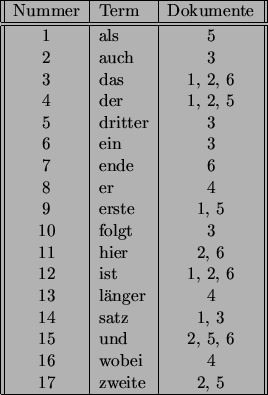
\includegraphics[scale=0.5]{../Abbildungen/index.png}
	\caption{Beispiel für einen invertierten Index \cite{index_Uni_Munich}}
\end{figure}

\subsection{Umsetzung eines invertierten Index}
Nachdem das Prinzip des invertierten Index klar ist, steht die Frage im Raum wie dieser umgesetzt werden kann.
Es liegt nahe als Datenstruktur einen Trie einzusetzen. Ein Trie ist ein spezieller Suchbaum, welcher besonders gut zum Suchen von Zeichenketten geeignet ist \cite{IR_Intro_Cambridge}.
\newline
Alternativ kann über den Einsatz einer Hasmap nachgedacht werden, jedoch führt dies zu folgendem Problem:
Angenommen eine vom Nutzer eingegebene Query ist nicht in der Hashmap vorhanden. Die Hash-Funktion wird einen Fehler werfen. Da in einer Hashmap Wörter, die ähnlich zueinander sind, nicht unbedingt benachbart gespeichert werden und keinerlei Information darüber bekannt ist, wo zur Query ähnliche Wörter gespeichert sind, kann im Falle, dass ein oder mehrere Wörter der Query nicht vorhanden sind, nicht mit geringem Aufwand nach ähnlichen Wörtern gesucht werden. Bei Tries besteht dieses Problem nicht \cite{IR_Intro_Cambridge}. 
\newline
Da in der Beispielimplementierung ein Trie als Datenstruktur zum Einsatz kommen wird, soll diese kurz vorgestellt werden.

\subsubsection{Tries}
Ein Trie wird auf der Basis einer Menge von Zeichenketten aufgebaut. Jede Zeichenkette, die gefunden werden muss, ist innerhalb des Tries repräsentiert.
\newline
Erreicht wird dies dadurch, dass ein Knoten jeweils ein Zeichen repräsentiert und eine Liste mit Verweisen auf die nächsten möglichen Knoten hält, basierend auf einem weiteren Zeichen.
Die folgende Abbildung zeigt einen Trie.

\begin{figure}[H]
	\centering
	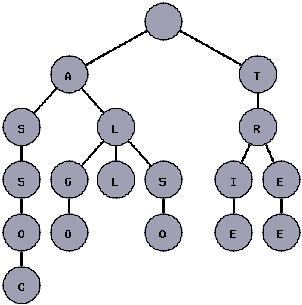
\includegraphics[scale=0.7]{../Abbildungen/trie.png}
	\caption{Beispiel eines Tries \cite{trie_Abb}}
\end{figure}

\newpage
Im Folgenden soll eine formale Definition eines Tries gegeben werden:
\newline
\begin{defi}
	Sei $\sum$ eine endliche Menge von Zeichen (Alphabet) und $\sum^{*}$ die Menge aller Wörter, die über $\sum$ gebildet werden können. Sei $S$ $\subseteq$ $\sum^{*}$. Dann ist $T = (V, E)$ ein Trie, wobei $V$ die Menge aller Knoten und $E$ die Menge aller Kanten ist. Darüber hinaus muss gelten:
	
	\begin{itemize}
		\item $\forall e \in E: e$ ist mit Zeichen aus $\sum$ beschriftet.
		\item $\forall v \in V:$ alle ausgehenden Kanten von $v$ sind unterschiedlich beschriftet mit einem Zeichen $z \in \sum$
		\item $\forall S_i \in S: \exists v \in V: S_i$ ist ein Präfix der Konkatenation der Beschriftungen des Pfades vom Wurzelknoten bis $v$.
		\item $\forall b \in V: \exists S_i \in S:$ Die Konkatenation der Beschriftungen von der Wurzel bis $b$ ergibt $S_i$, sofern $b$ ein Blatt des Tries ist.
	\end{itemize}
\end{defi}

Definition 2.7 ist aus \cite{Trie_wiki} entnommen.
\newline \newline
Das Suchen nach gespeicherten Wörtern gestaltet sich nun verhältnismäßig einfach: Um das Wort \glqq Tree\grqq im, in der Abbildung gezeigten, Trie zu finden, wird wie folgt vorgegangen.
\newline 
Stellt der User die Anfrage \glqq Tree\grqq wird diese Query nun Zeichen für Zeichen durchgegangen. Beginnend bei \glqq T\grqq wird im Wurzelknoten geprüft, ob es einen Verweis auf einen Knoten gibt, der ein \glqq T\grqq repräsentiert \cite{trie_Abb}. Existiert ein solcher Knoten, wird in diesem geprüft, ob es einen Knoten gibt, der das nächste Zeichen in der Query (das \glqq r\grqq) repräsentiert. Ist dies der Fall wird das Verfahren solange wiederholt bis die Query komplett eingelesen ist oder in der Query ein Zeichen steht, das durch keinen Knoten im Trie repräsentiert ist \cite{trie_Abb} \cite{Trie_Blog}.
\newline \newline
Ähnlich leicht funktioniert das Einfügen neuer Wörter in den Trie. Dazu wird - wie beim Suchen - das Wort, das eingefügt werden soll, so weit wie möglich nach dem oben beschriebenen Muster eingelesen und es wird zu den entsprechenden Knoten gesprungen \cite{trie_Abb} \cite{Trie_Blog}. Wird nun ein Zeichen eingelesen, das nicht durch einen Knoten repräsentiert ist, wird ein neuer Knoten erzeugt, welcher dieses Zeichen repräsentiert \cite{trie_Abb}. Alle nun noch einzulesenden Zeichen erhalten einen neuen Knoten, da der neu erzeugte Knoten natürlich nicht auf bereits vorhandene Knoten zeigen kann. Innerhalb dieses Knotens wird eine Liste angelegt, die Verweise auf weitere Knoten hält \cite{trie_Abb}. In dieser Liste wird ein Verweis auf den Knoten angelegt, der das nächste Zeichen des einzufügenden Wortes repräsentiert. Dieses Verfahren setzt sich solange fort, bis das neue Wort vollständig eingelesen ist.
\newline \newline
Das Löschen soll in diesem Rahmen nicht aufgezeigt werden, da dies weitaus komplexer sein kann als das Finden oder Einfügen von Einträgen.
\newline \newline
Ein Knoten, zu dem man mit dem Wort $S_i$ gelangt, muss außerdem eine Liste mit Verweisen auf alle Dokumente, in denen das Wort $S_i$ vorkommt, speichern. Gibt es keine Dokumente, in denen $S_i$ vorkommt, ist die Liste leer.

\section{Komprimierung des Index}
Bei großen Dokumentenmengen wächst die Größe des Index ebenfalls. Doch nicht nur die Größe des Index wächst, sondern auch die benötigte Zeit, um auf eine Query zu antworten \cite{IR_Intro_Cambridge}.
Die Index-Komprimierung adressiert genau dieses Problem. Über die Jahre der Forschung haben sich einige Komprimierungs-Techniken bewährt und sind bei den allermeisten aktuellen Suchmaschinen in Benutzung. \newline
Dieser Abschnitt soll das Thema Komprimierung erläutern, das Hauptaugenmerk liegt dabei auf der Komprimierungs-Technik, die in der Beispielimplementierung eingesetzt wird.

\subsection{Nutzen der Komprimierung}
Bevor die technischen Details der Komprimierung betrachtet werden, sollen zunächst die Vorteile, die sich durch die Komprimierung ergeben, aufgezeigt werden.
\\
In erster Linie wird durch die Komprimierung Platz auf dem Speichermedium, auf dem der Index liegt, gespart. Liegt dieser beispielsweise in einer Datei auf einer Festplatte, zieht die Komprimierung noch weitere Vorteile mit sich: Bei Schreib- bzw. Leseoperationen auf die Datei, müssen durch die Komprimierung weniger Bytes vom Hauptspeicher zur Festplatte bzw. umgekehrt, transportiert werden. Dadurch verringert sich die I/O-Zeit \cite[S. 58, 86]{IR_Intro_Cambridge}. Weiter kann ein größerer Teil des Indexes im Cache gehalten werden, was den Zugriff auf den Index beschleunigt, da weniger I/O-Operationen auf der Festplatte erforderlich sind \cite[S. 58, 86]{IR_Intro_Cambridge}.

\subsection{Dictionary komprimieren}
In \ref{txt:inverted_index} wurde beschrieben, dass sich der invertierte Index in das Dictionary und die Posting-Listen aufteilt.
Dies sind die beiden Punkte, an denen bei der Komprimierung angesetzt werden kann.
Die erste Möglichkeit, die genauer betrachtet werden soll, ist die Dictionary-Kompression.
Der Idee, die betrachtet werden soll, liegt zugrunde, dass in der Datenstruktur, die zur Suche der Wörter, die in der Query enthalten sind, genutzt wird, in jedem Knoten ein Zeichen gespeichert wird. Wird UTF-8 zur Zeichencodierung verwendet, fällt pro Zeichen mindestens $1$ Byte an, das in jedem Knoten gespeichert werden muss. Meist besteht ein in UTF-8 codiertes Zeichen jedoch aus mehr als einem Byte. \\
Eine Möglichkeit, Speicherplatz zu sparen, ist, nicht ein Zeichen pro Konten zu speichern, sondern lediglich einen Pointer auf ein Zeichen. Der Pointer wird als Index auf eine Liste verwendet, welche alle Zeichen enthält, die in den Dokumenten, die der Index \glqq kennt\grqq. Ist die dem Index zugrunde liegende Datenstruktur ein B-Baum oder ein Binärbaum, kann noch weiter Speicherplatz gespart werden, indem der Liste Teilstrings hinzugefügt werden, die in mehreren Wörtern vorkommen. Da im Rahmen dieser Arbeit jedoch ein Trie verwendet wird, wird dieser Punkt nicht weiter betrachtet, da ein Trie eine solche Komprimierung bereits liefert, da jeder Substring lediglich ein mal abgespeichert wird.
\\
\\
Ein Beispiel soll aufzeigen, wie mittels Pointern Speicherplatz gespart werden kann. Dazu zunächst eine Rechnung, wie viel Speicherplatz durch Zeichen in einem klassischen Trie benötigt wird:
Sei $T_1$ ein Trie mit einer Knotenzahl von $15$ Knoten. Jeder der Knoten beinhaltet ein Zeichen, welches jeweils $2$ Byte benötigt. Somit werden $15 \ * \ 2 \ = \ 30$ Byte benötigt, um alle Zeichen zu speichern. 
\\
Wird nun die Dictionary-Komprimierung angewendet, so wird eine Liste mit allen Zeichen, die in den eingelesenen Dokumenten vorkommen, angelegt. Die Größe dieser Liste bleibt beim Hinzufügen neuer Dokumente in den Index konstant, sofern die Dokumente keine bisher unbekannten Zeichen beinhalten. Die Größe der Liste ist somit für große Tries, wie sie in einem Index gewöhnlicherweise entstehen, vernachlässigbar. 
\\
Die Liste $l$ habe $26$ Einträge und beinhaltet das Alphabet von a-z ohne Umlaute.
Jeder Knoten im Trie muss jetzt lediglich einen Zeiger auf einen Listeneintrag abspeichern. Damit werden nur noch $log_2(26) \approx 4,7$ Bits benötigt. Da aufgerundet werden muss, werden 5 Bits zum Speichern des Zeigers benötigt. Damit wird eine Einsparung von $11$ Bits pro Knoten erreicht, wodurch im gesamten Trie $T_1$ $11 \ * \ 15  \ = \ 165$ Bits eingespart werden, was $20$ Bytes entspricht.
\\
Um noch weitere Zeichen in die Liste aufnehmen zu können, kann pro Zeiger ein Byte genutzt werden. Dadurch können $256$ Zeichen unterstützt werden und dennoch werden im Trie $T_1$ $15$ Bytes eingespart.
Dies wird Byte-Alignment genannt.
\\
In diesem Beispiel scheint sich der Nutzen der Komprimierung in Grenzen zu halten, betrachtet man jedoch einen Trie $T_2$ mit einer Knotenzahl von $10.000$, ergibt sich ein anderes Bild: 
Statt $10.000 \ * \ 2 = 20.000$ Byte werden mit Byte-Alignment nur noch $10.000$ Byte benötigt, wodurch $50\%$ Speicherplatz gespart werden, sofern der marginale Speicherbedarf der Liste $l$ nicht mit einbezogen wird.

\subsection{Postings-Liste komprimieren}
Weitaus mehr Speicher wird von den Posting-Listen benötigt, die im Index gespeichert werden müssen. Zur Erinnerung: Die Einträge in einer Posting-Liste verweisen auf diejenigen Dokumente, in denen das entsprechende Wort bzw. der entsprechende Term vorkommt.
\\
Der Speicherbedarf der Posting-Listen über den gesamten Index kann nicht so einfach berechnet werden, wie der Speicherbedarf des Dictionarys. Im Falle eines Tries lässt sich die Anzahl der benötigten Bytes für das Dictionary mit $ Anzahl \ Knoten \ * \ Bytes \ pro \ Zeichen$ berechnen. Da die Posting-Listen jedoch unterschiedliche Längen pro Knoten aufweisen, lässt sich keine solch einfach Formel finden.
\\
Durchschnittlich benötigen Posting-Listen mehr Speicher pro Knoten als die Byteanzahl eines zu speichernden Zeichens. Werden die Dokumenten-IDs (oder Postings) mit 4-Byte-Integern abgespeichert, benötigt eine Liste $l$ $|l| \ * \ 4$ Bytes. mit 4-Byte-Integern können auf $2^{32}$ Dokumente referenziert werden, was bei großen Dokumentenmengen schnell zu Problemen führt, da weit mehr Dokumente im Index aufgenommen werden müssen. Werden 8-Byte-Integer genutzt, so können $2^{64}$ Dokumente referenziert werden, die Posting-Liste $l$ benötigt dann $|l| \ * \ 8$ Byte.
\\
Werden in der Liste statt der echten Dokumenten-ID lediglich die Differenzen zwischen den einzelnen Einträgen gespeichert, können kleinere Zahlen genutzt werden. Die folgenden zwei Tabellen zeigen, wie das aussehen könnte:


\\
Kleinere Zahlen können mit weniger Bits codiert werden, wie dies umgesetzt wird, ist Gegenstand der nächsten Abschnitte.
Es gibt mehrere Verfahren, wie diese Liste komprimiert werden kann bzw. die Integer-Werte, die in der Liste enthalten sind. Es wird dabei zwischen byte- und bit-orientierten Codes unterschieden. Im Folgenden werden zwei Varianten vorgestellt, Variable Byte Encoding und $\gamma$-Codes.

\subsubsection{Variable Byte Encoding (VBE)}
Dieser Code fällt - wie der Name bereits zeigt - in die Kategorie der byte-orientierten Komprimierung.
\\
In den meisten Computersystemen werden Integer als 4-Byte-Integer dargestellt.
Wie oben gezeigt, müssen jedoch nur noch kleine Zahlen gespeichert werden. Es wäre Verschwendung, kleine Zahlen, die mithilfe ein oder zwei Bytes codiert werden können, als 4-Byte-Integer abzuspeichern, bei dem zwei Byte lediglich führende 0en darstellen.
\\



\section{TF-IDF Gewichtung}


\section{Retrieval}
%---------------------------------------------------------------------------------
	%Literaturverzeichnis
	\pagestyle{plain}
	\printbibliography
%---------------------------------------------------------------------------------	
\end{document}
%#################################################################################